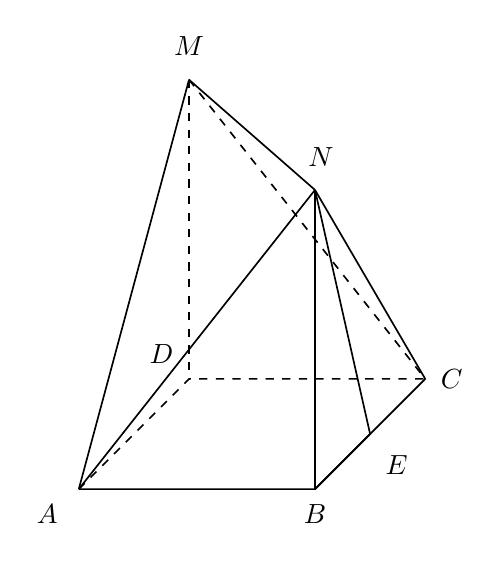
\begin{tikzpicture}[x=1cm,y=1cm,line width=.6pt,font=\normalsize]
% Schematic two-pillar configuration over square base
\coordinate (A) at (0,0);
\coordinate (B) at (3,0);
\coordinate (C) at (4.4,1.4);
\coordinate (D) at (1.4,1.4);
\coordinate (M) at (1.4,5.2);
\coordinate (N) at (3,3.8);
\coordinate (E) at (3.7,0.7);
% base
\draw (A)--(B)--(E)--(C);
\draw (B)--(E);
\draw[dashed] (A)--(D)--(C);
% pillars and top
\draw (A)--(M);
\draw[dashed] (M)--(D);
\draw (M)--(N);
\draw[dashed] (M)--(C);
\draw (N)--(B);
\draw (N)--(A);
\draw (N)--(C);
\draw (N)--(E);
% labels with clearance
\node[anchor=north east,xshift=-4pt,yshift=-2pt] at (A) {$A$};
\node[anchor=north,yshift=-2pt] at (B) {$B$};
\node[anchor=west,xshift=2pt] at (C) {$C$};
\node[anchor=south east,xshift=-2pt,yshift=2pt] at (D) {$D$};
\node[anchor=south,yshift=5pt] at (M) {$M$};
\node[anchor=south west,xshift=-6pt,yshift=5pt] at (N) {$N$};
\node[anchor=north west,xshift=2pt,yshift=-4pt] at (E) {$E$};
\end{tikzpicture}
